\chapter[Literature Review]{Literature Review}

\section{History of Vue.js}
Vue was created by Evan You whilst working at Google on a UI-heavy project \cite{macrae2018vue}. Prior to the creation of Vue, there were no frameworks for rapidly prototyping UI interfaces. Subsequently, You, who did not find any viable solutions to his problem started working on his own. Angular, already widely used by developers and created by Google itself was too big and bloated of a framework to be sensible for small applications. React, a fairly new framework at the time also proved being too complex just like Backbone.js which was used for large-scale enterprise applications. None of these frameworks were adequate for prototyping \cite[p.~10]{filipova2016learning}. You's approach of reactive data-binding and reusable components later named Vue.js, was realeased in February 2014 \cite{macrae2018vue} and helped fill that niche. Gradually improved over the years Vue is now utilized for complex enterprise-grade applications and small prototpyes alike and has since been adopted by many developers and companies around the world. The most noteworthy of which are: Facebook, Netflix, Adobe, Xiaomi, Alibaba and GitLab \cite{CompaniesUsingVue:online}. With more than 130,000 stars on GitHub at the time of this writing, Vue is more popular than both React (122,000 stars) and Angular (45,000 stars).


\section{Comparison to other Frameworks}
As there is an excessive amount of libraries and frameworks available for creating web based applications this section will be limited to comparing Vue to the other most popular frameworks React and Angular.

\textbf{Glossary:}

Basic Usage: How this particular framework / library is typically used with a bundler / build process

Scaling: scaling in terms of functionality rather than how many developers are actively working on a project or the number of end users using the application. 

Flexibility of a framework / library: flexibility in terms of how opinionated it is

% VUE

\subsection{Vue}

\subsubsection{Basic Usage}
Vue.js is a JavaScript framework which "makes it easier for developers to create rich, interactive websites" \cite{macrae2018vue} which is based on a virtual DOM \cite{ComparisonVue:online}. A virtual DOM is a set of instructions that are followed when a user interface is updated \cite[p.~81]{LearningReactBanks:book} creating a new layer between the Browsers DOM and Vue, drastically increasing efficiency in the process \cite{LearningReactBanks:book}. By default any valid HTML can be used to define the basic structure of Vue components, which is also referred to as a "template" in Vue terminology. Component-scoped data and logic are defined within the script tags and are complemented by functional directives such as "v-if" inside the template. Style sheets are defined within style tags, separating style and logic. By optionally using the scoped keyword, css is bound to a specific component, reducing the risk of polluting global style sheets. The composition of template, script and style tags is called a "Single File Component", indicating that only a single file needed used to create a functional and styled component. Additionally, props provide a uni-directional way of passing data from a parent component to a child component, whereas events are commonly used to pass data in the opposite direction. "Methods" can be defined to execute repeatable code, "computed properties" are a powerful way of reflecting changes of data and "watchers" behave like computed properties but only execute code upon data changes without returning a data type. In


The following code sample illustrates how Vue is typically used: \newline
\begin{lstlisting}[caption=Vue Template, captionpos=b, style=htmlcssjs]{Vue Single File Component}
<template>
<div>
<h1 v-if="condition" class="custom-title"> Hello {{ user }} </h1>
<h1 v-else> "Hello Stranger" </h1>
</div>
</template>

</script>
export default {
    data: {
        return() {
            user: "Alex"
        }
    },
    methods: {/*execute code*/},
    computed: {/*return data when data changes*/},
    watch: {/*execute code when data changes*/}
}
</script>

</style scoped>
.custom-title {
    size: 30px;
}
</style>
\end{lstlisting}

\subsubsection{Scaling}
Vue applications can easily be scaled up or down in terms of application functionality depending on the requirements. In order to create sophisticated and large applications, three parts have to be incorporated in general: The core library, routing and state management, of which all are officially provided by Vue as supporting libraries \cite{ComparisonVue:online}. This typically goes along with bundling tools such as Webpack or Browserify, which make for a much more powerful development environment. In addition, Vue offers an optional CLI generator interface for scaffolding projects, leaving the choice to the developer which building system and plugins to use. Using this interface, sophisticated applications along with routing and state management can be created. If the goal is to add reactive and interactive elements to an existing webpage, Vue can be used by adding a script tag to the site on which it is used \cites{AddingReact:online, ComparisonVue:online}. In doing so, no bundler is necessary for code to function but at the same time developers are deprived from being able to use plugins, preprocessors, and various other tools and are most commonly left with a larger bundle size \cite{ComparisonVue:online}.

\subsubsection{Performance \& Build Size}
The bundle size of a typical Vue project with the additional dependencies of vuex (state-management) and vue-router is about ~30KB \cite{ComparisonVue:online}. As for performance, Vue resides in the upper category in terms of startup time, memory allocation and rendering time \cite{FrameworksPerformance:online}, due to the usage of a virtual DOM. Early beta versions of Vue 3.0 even reduce memory allocation and rendering time by about 50\%.

\subsubsection{Flexibility \& Learning Curve}
Among other things, Single File Components are easy to use when coming from an HTML background, make transitioning existing applications to Vue smoother, do not have a steep learning curve resulting in faster adoption by beginners and can be further enhanced with various preprocessors \cite{ComparisonVue:online}. As Vue supports various bundlers and build systems while not enforcing specific ways of usage, you could argue that it is less opinionated than some other technologies. 

% REACT

\subsection{React}

\subsubsection{Basic Usage}
React describes itself as a "library for building user interface", which does not automatically come with as much functionality a traditional framework would have \cite[p.~2]{LearningReactBanks:book}. Like Vue it also utilizes a virtual DOM \cite[p.~81]{LearningReactBanks:book}. In React everything is defined in terms of JavaScript, meaning HTML often coupled with CSS are directly embedded into so called render functions. JSX, which is essentially a syntax extension to JavaScript \cite{ReactJSX:online} is most commonly used (even though not necessary) to define these render functions and is capable of mixing the full power of a programming language with rendering and UI logic \cite{ComparisonVue:online}. Styling is most commonly achieved by CSS-in-JS solutions provided by additional libraries, consolidating logic and styling in the same place \cite{islam2017reactjs:article}. \newline

\begin{lstlisting}[caption=Usage of JSX Render Function, captionpos=b, style=htmlcssjs]{Usage of JSX Render Function}
class Welcome extends React.Component {
    render() {
        return <h1>Hello, {this.props.name}</h1>;
    }
}
\end{lstlisting}

In addition, JSX render functions provide:
\begin{itemize}
    \item full leverage of JavaScript, including temporary variables and direct references to these
    \item and good tooling support (linting, type checking, autocompletion) \cite{ComparisonVue:online}.
\end{itemize}

\subsubsection{Scaling}
Like Vue React can either be used with a bundler or added to a single site by using a script tag. React outsources routing and state management to the community, fragmenting its ecosysytem in the process \cite{ComparisonVue:online}. More than eleven well-known routing libraries are available for React with similar statistics for state management and styling which gives developers a vast variety of available options but also makes choosing the right library for a projects requirements a much more tedious task. Reacts cli "create-react-app" works in a similar fashion like Vues but is much more limited: instead of letting the user choose a variety of options, it assumes that a single page application is to be created with always the same dependencies.

\subsubsection{Performance \& Build Size}
The React source itself has about 4.7KB gzipped which makes sense, given that React advertises itself as a library rather than a framework. However, including React DOM (34KB), routing with react-router (6.9KB) and state management with redux (2.4KB) the total size grows considerably to 48KB. Performancewise, React can also be categorized as a library of the upper category \cite{FrameworksPerformance:online} due to the usage of a virtual DOM.

\subsubsection{Flexibility \& Learning Curve}
To take advantage of online resources and documentation JSX is almost a requirement. As it is an extension to JavaScript, developers who are familiar with this programming language can easily learn the additional syntax \cite{ReactJSX:online}. Without prior knowledge of JavaScript, the learning curve rises considerably. The availability of various libraries makes React a very flexible library, given that the core of react is so slim and additional functionality is to be added by using those. 
% Even though using JSX is the recommended approach for developing React applications, JavaScript can be used instead


% ANGULAR
\subsection{Angular}

\subsubsection{Basic Usage}
Even though JavaScript could be used, Angular essentially requires the usage of TypeScript, a typed superset of JavaScript \cite{TypeScript:online}. As opposed to JavaScript, TypeScript comes with static type checking which naturally makes applications less prone to errors \cite{DynamicallyTypedLanguages:proceedings} and therefore is often used within very large corporate projects. Like Vue Angular also uses a component-based approach for composing user interfaces, but rather than using a single file, multiple files for HTML, CSS and JavaScript logic are typically used, however, CSS and HTML can be inlined in Angular components.  \newline

\begin{lstlisting}[caption=Angular Basic Usage Example, captionpos=b, style=htmlcssjs]{Angular Basic Usage}
//app.component.html
<button (click)="show = !show">{{show ? 'hide' : 'show'}}</button>
show = {{show}}
<br>
<div *ngIf="show; else elseBlock">Text to show</div>
<ng-template #elseBlock>Alternate text while primary text is hidden</ng-template>

// app.component.ts
import { Component } from '@angular/core';

@Component({
  selector: 'app-root',
  templateUrl: './app.component.html',
  styleUrls: ['./app.component.css']
})

export class SampleComponent {
  show: boolean = true;
}
\end{lstlisting}

\subsubsection{Scaling}
Angular provides a lot of functionality out of the box. Designed with the purpose of building large and complex applications Angulars API exposes a lot of functionality which is most commonly only necessary for exactly these types of applications. It includes everything from routing, state management, http calls to complete testing suites, however, Angular can also be added to existing sites using a script tag, only providing core functionality.

\subsubsection{Performance \& Build Size}
Angular applications built with the angular project scaffolding interface angular-cli have around 65KB gzipped, double the space as the other two frameworks. As for performance, Angular is also a performant framework \cite{FrameworksPerformance:online} but becomes slow under certain circusmstances: For instance if a project uses a lot of watchers and data in the scope changes, all watches are re-evaluated again \cite{ComparisonVue:online}.

\subsubsection{Flexibility \& Learning Curve}
 Angulars very big ecosystem and API provide most needed functionality out of the box but at the same time limit its flexibility. What is more, by prodiving pre-defined ways of interacting with Angular, it inherently becomes opinionated and more difficult to master \cite{ComparisonVue:online}.


\subsection{Conclusio}
% USAGE
All three frameworks solve similar problems but are used in different ways. Vues Single File Components consolidate logic, styles and HTML in the same place, React can and is mosten often used in a very resemblant way if used with a CSS-in-JS approach, whereas the "Angular way" is to split these parts into separate files. 

% SCALING
Applications built with React or Vue can be easily scaled up or down depending on the application-requirements. Large applications typically need the core library, routing and state management. While all of these are officially provided by the Vue core team for Vue applications, React leaves routing and state management to the community \cite{ComparisonVue:online}. Vue and React both offer an optional CLI generator interface to scaffold projects, however, Vue offers more options, leaving the choice to the developer which building system and plugins to use. React's more limiting approach with create-react-app makes it easier to start a project as it only needs a single dependency but limits the user to a given setup, which can however, be moved to a more customized environment with little effort whereas Angular is completely set up for the development of very large projects and provides most functionality out of the box, scaling up is therefore not a big problem because developers can rely on most of the functionality already existing.

All three frameworks can be scaled down by adding script tags to any site \cite{AddingReact:online, ComparisonVue:online} which however removes the powerful building layer.

% PERFORMANCE & BUILD SIZE
Vue and React both are resemblant in terms of runtime performance, are based on a virtual DOM and are used for similar use cases while Angular is a much more heavy-weight framework regarding performance and size. 

% FLEXIBILITY & LEARNING CURVE
JSX as well as TypeScript are additional learning steps and can lead to decreased productivity in smaller projects. Being a dynamic language, JavaScript's ability to address quickly changing requirements makes it especially suitable for rapid prototyping \cite[p.~72]{DynamicallyTypedLanguages:proceedings}. By using very HTML-like components Vue is often easier to master than the other two frameworks as most developers have at least basic knowledge of HTML. Nonetheless, Vue makes it possible to use TypeScript if the need arises, paving the way for bigger projects \cite{VueTypeScript:online}. Angular is not very flexible in the sense that users can pick whatever supporting library they deem best and is said to be an opinionated framework which enforces the "Angular way". Such frameworks are "pragmatic, with a strong sense of direction" \cite{Bedell:Opinionated:article} often forcing very specific conventions upon its users, effectively restricting what a developer can to with a framework. This also means there is a steeper learning curve but once overcome, can lead to increased productivity \cite{ComparisonVue:online}.

% Kiviat Diagram
The following diagram does by no means reflect the properties of the given framework / library 100\% accurately as some of them are somewhat subjective (e.g flexibility) but shall rather illustrate the strengths and weaknesses of each in relation to another.

\newcommand\ColorBox[1]{\textcolor{#1}{\rule{2ex}{2ex}}}

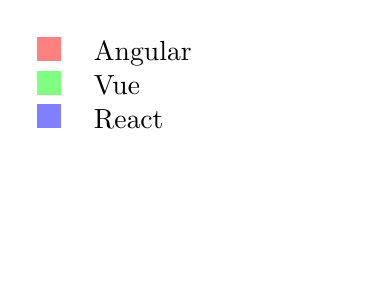
\begin{tikzpicture}
\tkzKiviatDiagram[scale=1,label distance=.5cm, radial=5, gap=1, lattice=5]
{Ease of Usage,Scaling,Performance,Build Size,Flexibility}
\tkzKiviatLine[thick, color=green, mark=none, fill=green!20, opacity=.5](5,3,4,4,4)
\tkzKiviatLine[thick, color=blue, mark=none, fill=blue!20, opacity=.5](4,4,3,3,4) 
\tkzKiviatLine[thick, color=red, mark=none, fill=red!20](2,5,2.5,1,2)    
% \tkzKiviatGrad[prefix=,unity=100,suffix=\ \texteuro](1)  
\node[anchor=south west,xshift=-60pt,yshift=40pt] at (current bounding box.south east) 
{
\begin{tabular}{@{}lp{3cm}@{}}
\ColorBox{red!50} & Angular \\
\ColorBox{green!50} & Vue \\
\ColorBox{blue!50} & React \\
\end{tabular}
};
\end{tikzpicture}


\section{SEO for Single Page Applications}
